\section{Comparaison avec la photo
assombrie}\label{comparaison-avec-la-photo-assombrie}

\begin{figure}[htbp]
\centering
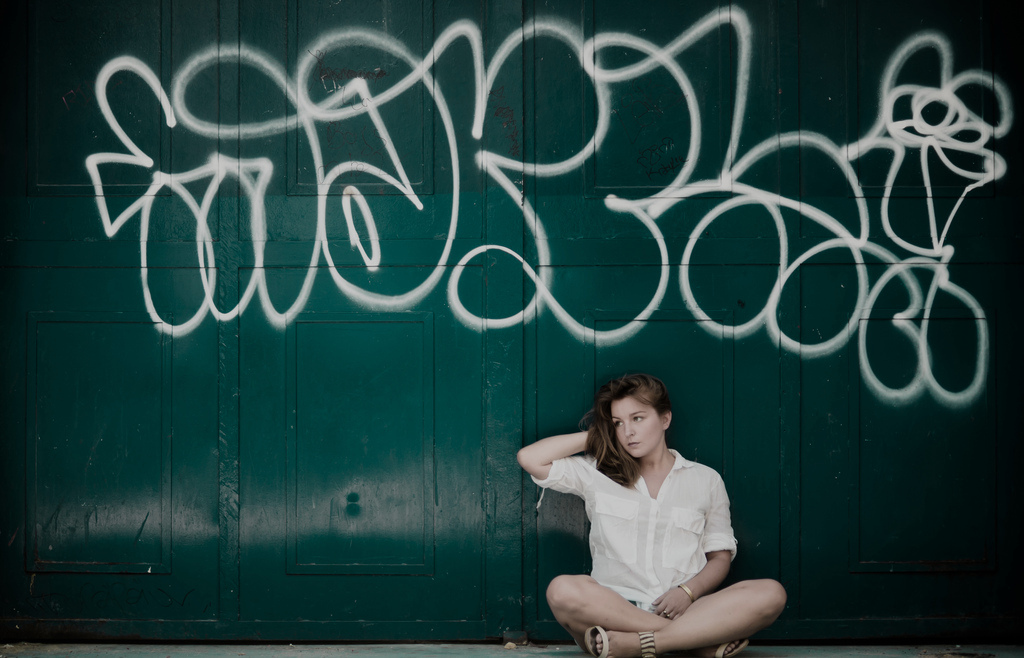
\includegraphics{../../photos/sombre.jpg}
\caption{Photo sombre}
\end{figure}

\begin{table}[htbp]
\centering
\begin{tabular}{llr}
\bfseries Formes &
\bfseries Bhattacharyya (\%)%
\DTLforeach*[\DTLiseq{\fichier}{photos/sombre.jpg}]{valeurs}{%
\fichier=Fichier, \formes=Formes,\bhatta=Bhattacharyya, \hue=Hue, \saturation=Saturation, \value=Value}{%
\\
\formes & \bhatta}
\end{tabular}
\end{table}

Comme pour la photo précédente, on peut considérer que les deux photos se
ressemblent, cependant elles n'ont pas le même niveau de ressemblance. En effet
celle-ci à une différence de $6.44 \%$ pour la colorimétrie par distance de
Bhattacharyya et de $12.6 \%$ pour les formes avec le filtre de Sobel. On peut
donc conclure que l'assombrissement de la photo n'a qu'un faible impact sur la
photo aussi bien d'un point de vue de la couleur que des formes.
